% ============================================================
% Plantilla IEEE para el informe final
% Compilar desde esta carpeta:
%   pdflatex main.tex
%   bibtex main
%   pdflatex main.tex
%   pdflatex main.tex
% ============================================================
\documentclass[conference]{IEEEtran}

\usepackage[utf8]{inputenc}
\usepackage[T1]{fontenc}
\usepackage[spanish]{babel}
\usepackage{amsmath,amssymb}
\usepackage{graphicx}
\usepackage{booktabs}
\usepackage{url}
\usepackage[hidelinks]{hyperref}

\graphicspath{{imagenes/}}

% ------------------------------------------------------------
% Datos del informe: completar o ajustar antes de entregar.
% ------------------------------------------------------------
\title{Simulación de eventos discretos de una línea de producción de muebles}

\author{
\IEEEauthorblockN{Victor Roa, Francis Valdiviezo, Cael Soto, Jimmy Ontaneda y Alejandro Padilla}
\IEEEauthorblockA{Carrera de Computación -- FEIRNNR\\
Universidad Nacional de Loja\\
Loja, Ecuador}
}

\begin{document}

\maketitle

\begin{abstract}
Se presenta un modelo de simulación de eventos discretos para una línea de fabricación
de muebles compuesta por las estaciones de corte, lijado, ensamblaje y acabado. El modelo
considera llegadas de Poisson, tiempos de servicio exponenciales, colas FIFO y un
operario por estación. Se ejecutaron 30 réplicas independientes de 1\,000 horas, con
100 horas de calentamiento, para estimar la utilización, la longitud de cola, el tiempo
de espera y el tiempo total de flujo. Los resultados se compararon con el modelo
analítico M/M/1 y con la Ley de Little. La estación de ensamblaje resultó ser el cuello
de botella de la línea base, con una utilización cercana al 75\,\%.
\end{abstract}

\begin{IEEEkeywords}
simulación de eventos discretos, SimPy, línea de producción, M/M/1, Ley de Little,
cuello de botella.
\end{IEEEkeywords}

% ============================================================
\section{Introducción}
% ============================================================
La simulación de eventos discretos permite representar sistemas de manufactura y
evaluar su desempeño sin intervenir el sistema real \cite{banks2010,law2015}. En una
línea de producción, las colas y los tiempos de espera dependen de la capacidad de cada
estación y de la variabilidad de las llegadas y de los tiempos de servicio
\cite{hopp2011}.

Este trabajo modela una línea de fabricación de muebles con cuatro estaciones en serie:
corte, lijado, ensamblaje y acabado. El objetivo es estimar sus indicadores de
desempeño, identificar la estación que limita la producción y comparar los resultados
con la teoría de colas M/M/1.

% TODO: completar el planteamiento del problema y la justificación.

% ============================================================
\section{Marco teórico}
% ============================================================
\subsection{Colas M/M/1}
Una estación M/M/1 tiene llegadas de Poisson, tiempos de servicio exponenciales, un
servidor y una cola FIFO sin límite \cite{gross2008}. Con
\(\mu_i = 60/t_i\) y \(\rho_i = \lambda/(c_i\mu_i)\), los indicadores teóricos son:

\begin{equation}
L_q = \frac{\rho^2}{1-\rho}, \qquad
W_q = \frac{L_q}{\lambda}, \qquad
W = W_q + \frac{1}{\mu}.
\end{equation}

\subsection{Ley de Little}
La Ley de Little relaciona la longitud media de la cola con la tasa efectiva de
llegadas y la espera media:

\begin{equation}
L_q = \lambda_{\text{ef}} \, W_q.
\end{equation}

\subsection{Error porcentual}
La diferencia entre la simulación y la teoría se reporta como:

\begin{equation}
\text{error}(\%) =
\frac{\left| x_{\text{sim}} - x_{\text{teo}} \right|}{x_{\text{teo}}} \times 100.
\end{equation}

% ============================================================
\section{Metodología}
% ============================================================
Se construyó un modelo de simulación de eventos discretos en Python 3.12 con SimPy
\cite{simpy2024,python2024}. La línea se representa como una secuencia de estaciones;
cada mueble ocupa un recurso, espera en una cola FIFO y avanza a la siguiente estación.
Los parámetros se leen desde archivos JSON y los resultados se guardan en CSV y PNG.

Se ejecutaron 30 réplicas independientes de 1\,000 horas por escenario. Las primeras
100 horas de cada réplica se descartaron como calentamiento, por lo que los indicadores
se calcularon sobre 900 horas. Cada réplica utiliza una semilla distinta derivada de
una semilla base, lo que permite reproducir los resultados.

% TODO: describir la organización del código y el procedimiento experimental.

% ============================================================
\section{Modelo de la línea}
% ============================================================
La línea base utiliza \(\lambda = 3\) muebles/h y un operario por estación. La
Tabla~\ref{tab:parametros} resume los tiempos medios de servicio.

\begin{table}[!t]
\centering
\caption{Parámetros de la línea base (E1).}
\label{tab:parametros}
\begin{tabular}{lcc}
\toprule
Estación & Operarios \(c_i\) & Tiempo \(t_i\) (min) \\
\midrule
Corte      & 1 & 8  \\
Lijado     & 1 & 10 \\
Ensamblaje & 1 & 15 \\
Acabado    & 1 & 12 \\
\bottomrule
\end{tabular}
\end{table}

La capacidad y la utilización de cada estación se calculan como:

\begin{equation}
C_i = c_i\mu_i, \qquad
\rho_i = \frac{\lambda}{c_i\mu_i}.
\end{equation}

El escenario E2 reduce el tiempo de ensamblaje a 12 min y el E3 lo reduce a 10 min.
Todos los escenarios conservan un operario por estación.

% ============================================================
\section{Resultados}
% ============================================================
La Tabla~\ref{tab:resultados} compara los indicadores simulados de ensamblaje y de la
línea con los valores teóricos. La producción se mantiene cerca de 3 muebles/h en los
tres escenarios.

\begin{table}[!t]
\centering
\caption{Resultados de ensamblaje y de la línea completa.}
\label{tab:resultados}
\begin{tabular}{lccc}
\toprule
Indicador & E1 & E2 & E3 \\
\midrule
\(\rho\) simulado / teórico & 75,1 / 75,0 & 59,8 / 60,0 & 49,7 / 50,0 \\
\(L_q\) simulado / teórico & 2,27 / 2,25 & 0,86 / 0,90 & 0,48 / 0,50 \\
\(W_q\) simulado / teórico (min) & 45,4 / 45,0 & 17,3 / 18,0 & 9,7 / 10,0 \\
Flujo simulado / teórico (min) & 124,0 / 123,3 & 92,2 / 93,3 & 82,2 / 83,3 \\
Producción (muebles/h) & 2,998 & 2,999 & 2,988 \\
Cuello de botella & Ensamblaje & Ensamblaje & Acabado \\
\bottomrule
\end{tabular}
\end{table}

\begin{figure}[!t]
\centering
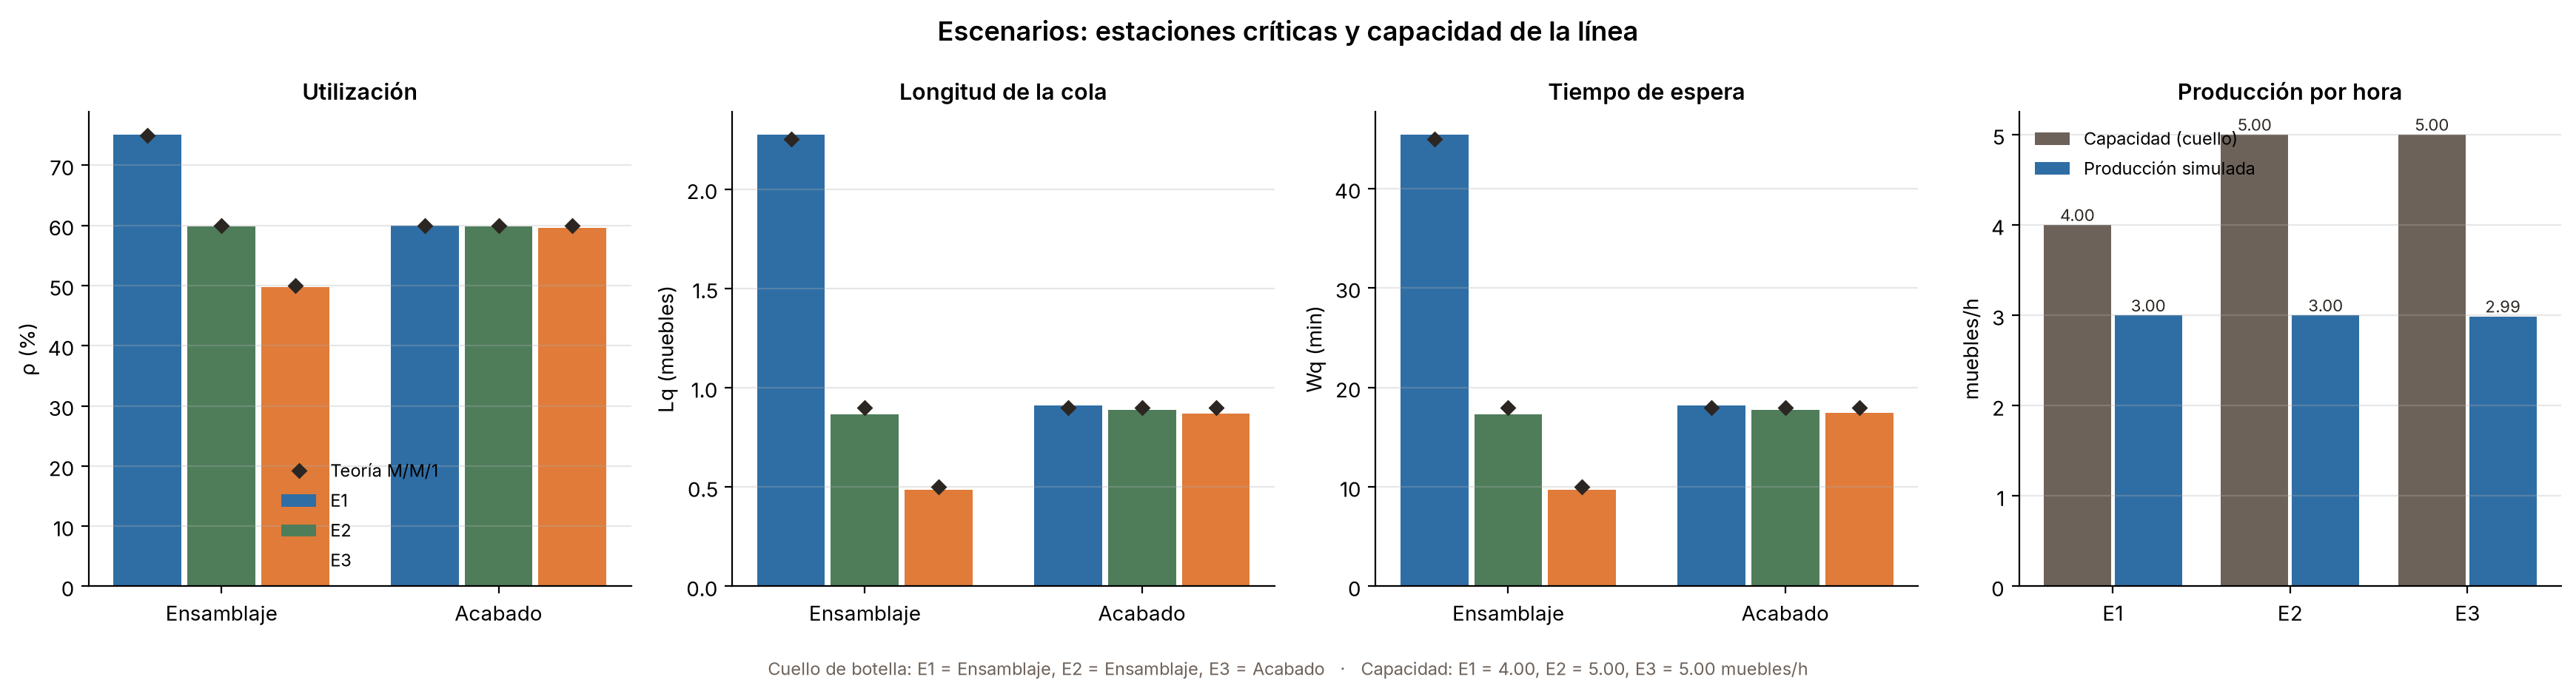
\includegraphics[width=\linewidth]{escenarios.png}
\caption{Comparación de utilización, cola y espera entre E1, E2 y E3.}
\label{fig:escenarios}
\end{figure}

\begin{figure}[!t]
\centering
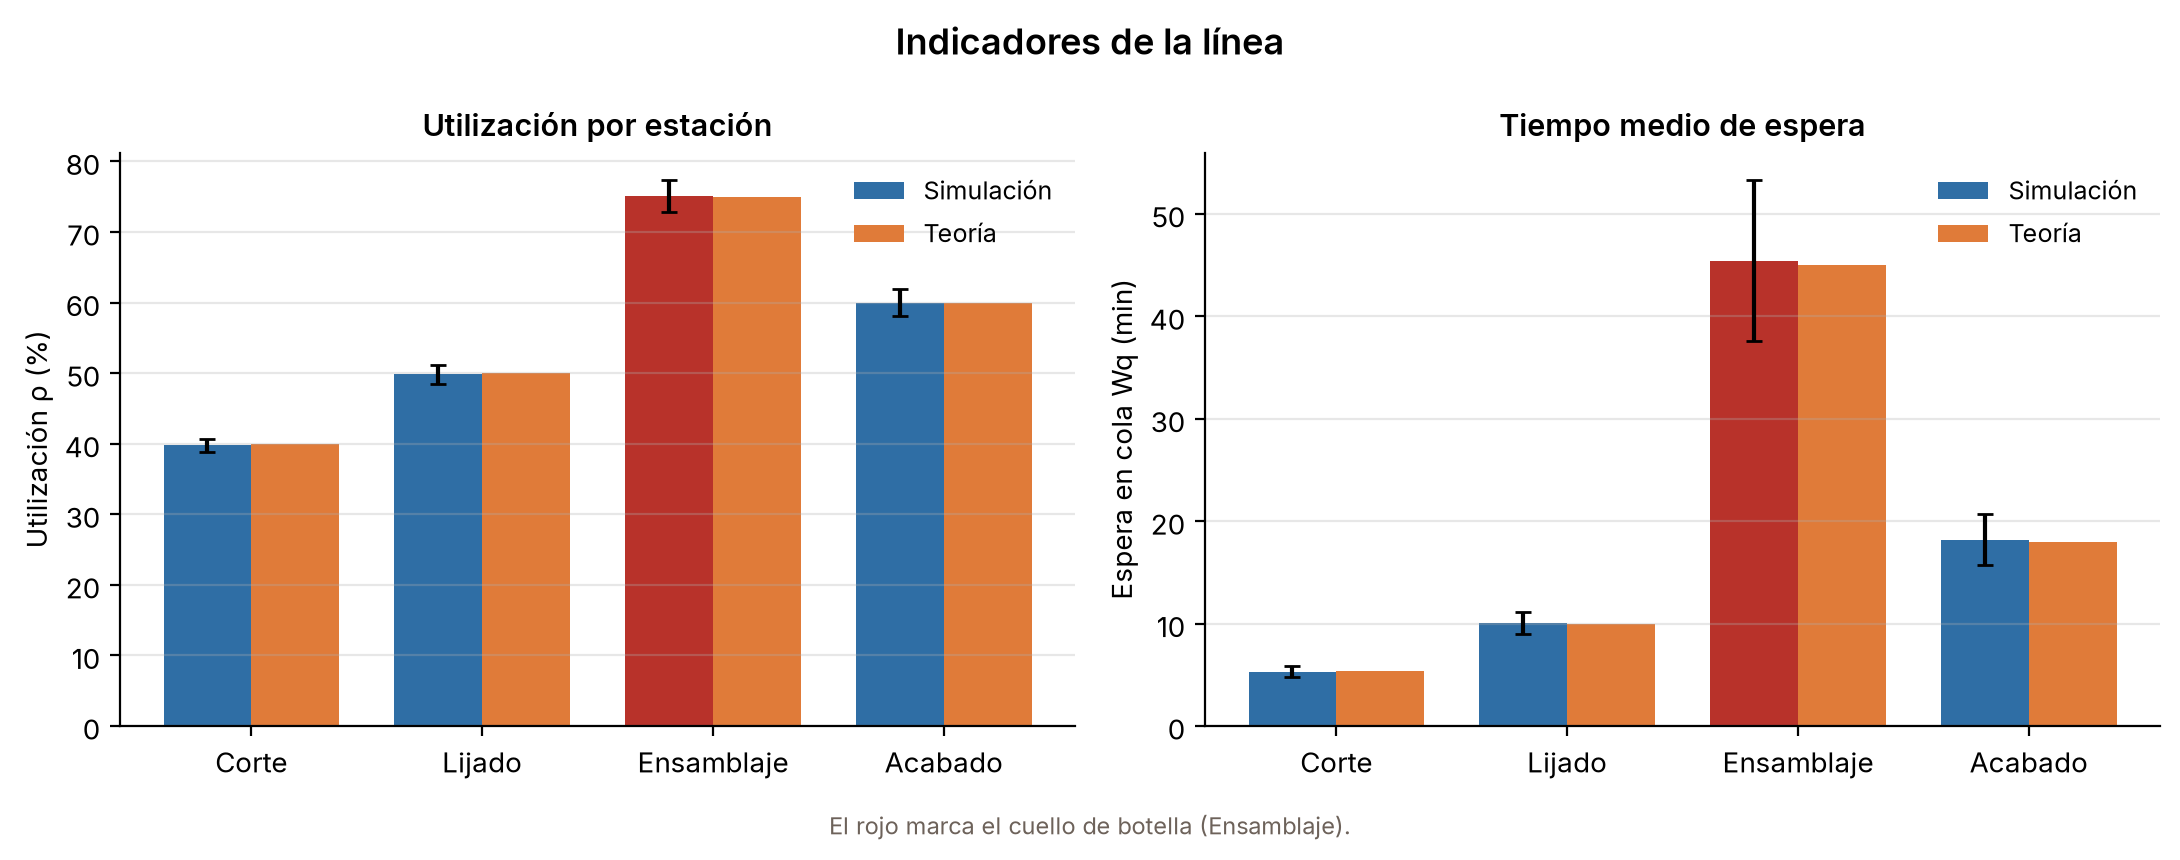
\includegraphics[width=\linewidth]{base.png}
\caption{Utilización y espera simuladas frente a la teoría M/M/1 en la línea base.}
\label{fig:base}
\end{figure}

\begin{figure}[!t]
\centering
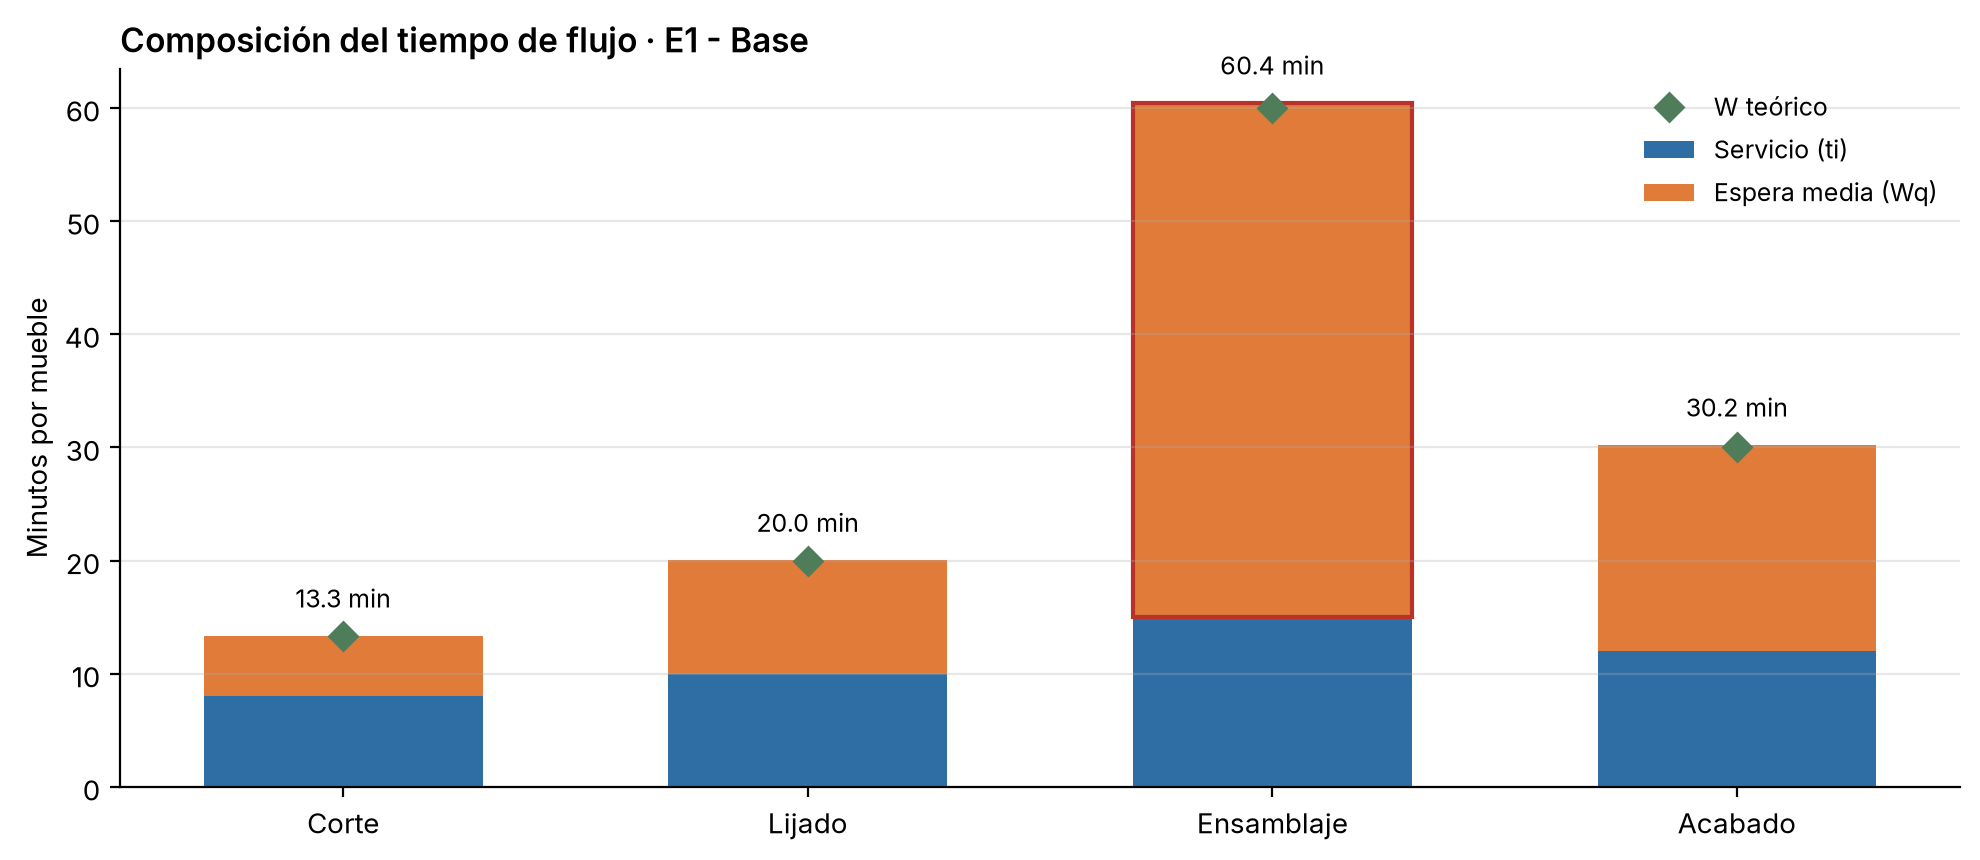
\includegraphics[width=\linewidth]{flujo-base.png}
\caption{Composición del tiempo de flujo en la línea base.}
\label{fig:flujo}
\end{figure}

% TODO: agregar las figuras de cola y distribución si el informe las necesita.
% Están disponibles en imagenes/ con los nombres cola-base.png,
% distribucion-cola-base.png, utilizacion-cola-base.png, etc.

% ============================================================
\section{Discusión}
% ============================================================
Los errores entre la simulación y la teoría M/M/1 son menores al 1,3\,\% en la línea
base. La estación de ensamblaje concentra la mayor utilización, la cola más larga y la
mayor espera, por lo que se identifica como el cuello de botella. Al reducir su tiempo
de servicio, la utilización baja y el cuello de botella se traslada a acabado en E3.

% TODO: relacionar estos resultados con los antecedentes y las fuentes citadas.

% ============================================================
\section{Conclusiones}
% ============================================================
El modelo de eventos discretos reprodujo los indicadores teóricos de la línea y permitió
identificar a ensamblaje como la estación que limita la producción en la línea base. La
comparación de escenarios muestra que reducir el tiempo de ensamblaje disminuye la cola
y el tiempo de flujo, aunque la producción se mantiene limitada por la tasa de llegadas.

% TODO: agregar recomendaciones y limitaciones del estudio.

% ============================================================
% Referencias
% ============================================================
\bibliographystyle{IEEEtran}
\bibliography{referencias}

\end{document}
